\documentclass[12pt]{article}

\usepackage{fullpage}
\usepackage{graphicx, rotating, booktabs} 
\usepackage{times} 
\usepackage{natbib} 
\usepackage{indentfirst} 
\usepackage{setspace}
\usepackage{grffile} 
\usepackage{hyperref}
\usepackage{adjustbox}
\usepackage{amsmath}
\setcitestyle{aysep{}}


\singlespace
\title{\textbf{Alliances: Force Multiplier or Foreign Entanglement?}}
\author{Joshua Alley\footnote{Graduate Student,
Department of Political Science, Texas A\&M University.}}
\date{{\normalsize \today}}

\bibliographystyle{apsr}

\begin{document}

\maketitle 

\newpage 

\doublespace 

\begin{abstract}
How does alliance participation change military spending? 
Some have argued that joining an alliance leads to greater defense expenditures while others contend that alliances lead to cuts in spending.
I argue both these views are correct under certain conditions; alliance participation can raise or lower growth in military expenditures, depending on treaty scope and state size. 
Because major powers use alliances and military spending to increase their influence in international relations and greater treaty scope provides more influence, treaty scope attenuates the usual positive correlation between alliance participation and military spending for major powers. 
Security-seeking non-major powers tend to reduce military spending as a result of alliance participation, but issue linkage bargaining in treaties with greater scope constrains this tendency. 
I test this argument by creating a measure of alliance treaty scope and employing that measure in a multilevel model. 
The research design generates new empirical evidence linking alliance participation and growth in state military spending from 1816 to 2007. 
I find that greater treaty scope increases growth in military spending in non-major powers and decreases spending growth for major powers.  
These results help scholars and policymakers better understand a central question about alliance politics that has been debated in scholarship for decades. 
\end{abstract}



\section{Introduction}


Scholars of international relations have long acknowledged that there are two ways for states to increase their security. 
States can invest in indigenous military capability or form alliances \citep{Morgenthau1948, Morrow1993}.
Because both policies provide security, broadly defined, alliance participation should change how states invest in military capability. 
But exactly how alliances influence military spending remains unclear. 


Existing scholarship produces competing predictions and evidence on the question of alliance participation and military spending. 
One view, which I call the \textit{force multiplier perspective} expects alliance participation will reduce military spending \citep{Morrow1993, Conybeare1994, DigiuseppePoast2016}. 
The other view, which I label the \textit{foreign entanglement group}, predicts alliance participants will spend more on defense \citep{Diehl1994, MorganPalmer2006}. 
This paper addresses this theoretical and empirical division, clarifying when alliance participation leads to more or less defense spending. 
In doing so, it helps clarify a longstanding debate about alliance politics.


I argue that whether alliance treaty participation increases or decreases military spending depends on two factors: state capability and alliance treaty scope. 
Treaties with wider scope add depth to promises of military support by promising other forms of cooperation.
Greater treaty scope means the agreement covers multiple issues, such as further defense cooperation, international organizations, or economic ties.  
Changing treaty scope alters how alliance participation impacts military spending. 
How treaty scope alters the impact of alliance participation depends on state capability because major and non-major power states use alliances and military spending for different purposes. 


Major powers use a mix of alliances and military spending to increase their influence--- shaping international relations to match their interests.
When major powers form alliances, they often increase their military spending to support the treaty and uphold their influence. 
Increasing treaty scope reduces this positive correlation between alliance participation and military spending for major powers, because scope gives major powers more influence through issue-linkages.
Thus, deep treaty commitments require less military spending for major powers to attain a particular amount of influence. 


Non-major powers use alliances and defense expenditures to ensure their territorial security.
Whenever possible, these states will rely on their allies for security, so alliance participation will often reduce growth in military spending.   
Increasing treaty scope constrains non-major powers tendency to reduce military spending through alliance participation. 
Adding further cooperation makes the treaty more valuable and gives partners greater influence through issue linkages. 
Thus, greater treaty scope will increase growth in non-major power military spending. 


I employ a novel research design to test my argument.
First, I develop a latent measure of alliance treaty scope. 
I then incorporate that measure into a multilevel model which estimates how specific alliance treaty characteristics modify the influence of alliance participation on growth in military spending.
I find that increasing treaty scope raises growth in non-major power military spending from alliance participation, and lowers growth in major power military spending from alliance participation. 


These findings have implications for our understanding of alliance politics and how international organizations shape domestic politics. 
How alliances shift growth in military spending has distributional consequences in international and domestic politics. 
In domestic politics, growth in military spending has opportunity costs--- funds spent on security cannot be spent on other goods. 
Greater military spending impacts economic growth \citep{ShinWard1999, AlptekinLevine2012} and domestic politics \citep{Narizny2003, WhittenWilliams2011, Williams2015}.
So alliances can shape domestic prosperity by shifting how resources are allocated to the military. 


In international politics, states bargain over distributing the costs and benefits of alliance participation.
Greater growth in military spending for some states and lower growth for others shifts the burden from maintaining the treaty. 
Distributing these costs and benefits through alliance formation and maintenance generates substantial tradeoffs for treaty members. 


My argument and findings indicate major and minor powers face different tradeoffs in alliance politics, however.
Deep commitments give major powers more influence but lead to greater entanglement abroad.
For non-major powers, deep treaties provide more security at the cost of freedom to reduce military spending. 
These tradeoffs shape treaty formation and maintenance, modifying the impact of alliance participation on military expenditures. 


Alliance politics tradeoffs for major and non-major powers illuminate two salient issues in US foreign policy. 
First, advocates of deep engagement \citep{Brooksetal2013} or restraint \citep{Posen2014} in US grand strategy should consider treaty scope in addition to whether the US should maintain its alliances. 
Second, debates about ``free-riding'' by US allies should engage more with the limited formal scope of most US treaties. 


The paper proceeds as follows. 
First, I summarize the competing arguments and mixed empirical evidence on alliance participation and military spending. 
Then I describe my state capability and treaty scope argument in more detail. 
The third and fourth sections present the research design and results. 
I then briefly use the argument to illustrate how formal NATO treaty commitments shaped military spending by the US and its allies. 
The final section concludes with a discussion of the results and implications for scholarship and policy.  


\section{Force Multiplier or Foreign Entanglement?}


% quick intro and straight into it
Scholarship on alliance participation and military spending is divided between force multiplier and foreign entanglement views.
Each perspective emphasizes different parts of alliance politics and contains multiple distinct arguments.  
First, I summarize the substitution and public goods logics connecting alliance participation with reduced defense spending. 


\subsection{Force Multiplier} 


All force multiplier arguments consider how alliances and military spending both provide security.
The first argument treats security from an alliance as a public good. 
\citet{OlsonZeckhauser1966} argue that alliances are subject to a collective action problem.
Because alliance security is neither rivalrous nor excludable, members contribute inadequate military spending. 
Each member ``free-rides'' on their partners, and smaller members exploit larger states. 
Spending less allows alliance members to consume more non-defense goods, but the alliance provides suboptimal security.\footnote{\citet{SandlerForbes1980, Oneal1990, SandlerHartley2001} all modify the public goods logic, but rely on Olson and Zeckhauser's basic intuition to understand alliance politics.} 


Another force multiplier argument focuses on substitution between foreign policy instruments.
Substitution arguments recognize that states can employ one policy in place of the other \citep{MostStarr1989}.  
Alliances provide security that states could not achieve without additional military spending \citep{Morrow1993, Conybeare1994}. 
Given extra security from a treaty, states can rely on their allies and and reallocate military spending to other goods. 


Under substitution, allied military capability replaces other members' defense expenditures. 
\citet{DigiuseppePoast2016} refine the substitution logic by arguing that states will only reduce spending if the alliance is credible. 
Because democracies make more credible commitments, they assert defense pacts with democracies will lower defense spending.


Both the substitution and public goods models expect alliance participation will reduce spending. 
The common thread between these arguments is the opportunity costs of military spending. 
Because spending more on the military leaves less for other goods \citep{Fordham1998}, states have incentives to rely on their allies for security. 
But the foreign entanglement group uses a different logic to argue alliance participation increases military expenditures. 


\subsection{Foreign Entanglement}


The foreign entanglement perspective contains a wide range of arguments, all with a common thread. 
In these arguments, states increase military spending to support their alliance commitments. 
Investing in military spending secures the foreign policy gains from alliance participation. 


% Crap ton of models- one sentance for each. add more detail later if needed. 
\citet{Diehl1994} argues that alliances increase foreign policy obligations, necessitating extra military spending. 
Because alliances expand what a state can achieve in international relations, states will increase military spending to pursue other foreign policy goals \citep{MorganPalmer2006}. 
\citet{Horowitzetal2017} show that buffer states increase defense effort to make themselves a more attractive alliance partner. 
Others assert that alliances generate cooperation, leading to higher defense spending \citep{Palmer1990, QuirozFlores2011}.\footnote{
\citet{SeneseVasquez2008} assert military spending and alliances are part of a conflict spiral that produces simultaneous growth in military expenditures and alliance participation. 
This argument suggests that any correlation between alliances and military spending is driven by conflict behavior, not treaty participation.
}
Of course, these predictions of a positive correlation between alliance participation and military spending are at odds with the force multiplier perspective. 


\subsection{Mixed Evidence} 


Debate between force multiplier and foreign entanglement views of alliances could be settled by a preponderance of evidence for one prediction, but mixed empirical results reinforce the theoretical division.\footnote{
Because tests of the public goods model regress military spending as a share of GDP on GDP, I ignore most tests of that theory while summarizing prior results. That research design suffers from an identification problem.}
Some studies find a positive association between alliance participation and military spending. 
Others find a negative relationship. 


% Specific and general studies
General studies of military spending and alliances compare many states through dummy indicators of alliance participation. 
This design captures a wide range of state-year observations and compare states with an alliance to those without.
Dummy indicators of alliance participation in a general study combine diverse treaties in a state-level measure. 
\autoref{tab:results-sum} summarizes previous results from general models of alliance participation and military spending. 
There are two negative, four positive and two null estimates of the correlation between alliance participation and spending. 


\begin{table}[hbt!]
\begin{center}
\begin{tabular}{lccc}
     & Decrease & Increase & Null \\
\hline
\citet{MostSiverson1987} &  &  & X \\
\citet{Conybeare1994} & X & &  \\
\citet{Diehl1994} &  & X &  \\
\citet{Goldsmith2003} &  &  & X \\
\citet{MorganPalmer2006} &  & X & \\ 
\citet{QuirozFlores2011} &  & X &  \\ 
\citet{DigiuseppePoast2016} & X &  & \\ 
\citet{Horowitzetal2017} &  & X & \\ 
\hline
\end{tabular}
\caption{General Findings of Association Between Alliance Participation and Military Spending.}
\label{tab:results-sum}
\end{center} 
\end{table}


% Virtues and shortcomings- Specific studies of substitution theory of FP 
Besides these general results, specific research designs detail individual treaties. 
Specific studies usually estimate how states respond to the military spending of a key ally. 
Most support for force multiplier arguments comes from specific designs \citep{BarnettLevy1991, Morrow1993, Sorokin1994, PluemperNeumayer2015}. 
But other specific studies find increased spending by alliance members \citep{ConybeareSandler1990, Chenetal1996}. 
Many of these designs focus on NATO and all suffer from a potential lack of generalizability. 


\subsection{Theoretical and Empirical Challenges}


Mixed empirical results reflect related theoretical and empirical challenges. 
Theoretically, both perspectives ignore valuable insights from the other.  
Foreign entanglement arguments contain useful insights about the need to support alliance commitments with additional military expenditures.
They ignore the opportunity costs of military spending, however. 


Force multiplier arguments capture the opportunity costs of military spending, but elide how defense spending supports alliances. 
As a result, the two perspectives have too little in common. 
Both treat alliances and their members as homogenous and emphasize different aspects of alliance participation. 
Opportunity costs and benefits of backing partners are not mutually exclusive aspects of military spending, however. 
The relative weight of these two issues will likely vary across states and treaties. 


% Mixed results due to alliance heretogeneity and changes over time. 
So far, scholarship on alliance participation and military spending has not paid enough attention to differences between alliance treaties and participants.
There is substantial heterogeneity among alliances.
Treaties vary in their obligations, membership, and capability. 
These differences between treaties mean alliance treaties have heterogeneous effects on conflict risk \citep{Leeds2003, Benson2012}. 
Alliance heterogeneity undermines binary measures of alliance participation in general studies and makes it difficult to infer general relationships from specific studies. 
 

Moreover, alliance members have different goals and constraints depending on their military capability.
Some states have extensive foreign policy ambitions, while others focus on defending their territory. 
The opportunity costs of military spending also vary across states. 
Therefore, the same alliance could have different effects on more or less capable members. 


My argument incorporates alliance heterogeneity and differences in member capability to explain how alliance participation is associated with military spending. 
I argue formal treaty scope alters the consequences of alliance participation for major and non-major powers. 
The next section summarizes the argument in more detail. 



\section{Argument}

% Focus on growth in spending
Before describing the logic of my argument, I must clarify the outcome of interest and its consequences for my claims. 
My argument predicts growth in military spending. 
Annual growth in spending is equal to changes in spending as a share of the previous year's budget. 
So growth in military expenditures is calculated as:
\begin{equation}
\mbox{Growth Mil. Expend} = \frac{ \mbox{Change Mil. Expend}_t }{ \mbox{Mil. Expend}_{t-1} }
\end{equation} 


Growth in spending is an appropriate quantity of interest. 
Benchmarking changes in spending to previous expenditures, incorporates the likely opportunity costs of annual spending changes for that state. 
Defense budgets are also subject to a ``ratchet effect'' \cite{Zielinskietal2017}, so increases in spending are rarely undone by corresponding cuts.
Especially for major powers, levels of military spending tend to rise over time. 
Theorizing about growth in spending provides clarity about the implications of alliance participation--- how much more or less would a state have changed their defense budget in the absence of a given treaty? 


Predicting growth in spending changes the interpretation of my argument and empirical findings. 
If a variable is positively or negatively associated with growth in spending, it may only change the level of military spending in a counterfactual sense. 
For example, lower spending growth need not imply falling levels of defense expenditures. 
Only negative growth in spending reduces the level of military expenditures. 
If a variable reduces growth, but the overall the level of growth remains positive, the level of military spending will still rise. 


Similarly, increasing expenditure growth does not indicate larger defense budgets. 
Only positive growth in spending increases the level of military expenditures. 
When increasing growth in military spending is relative to a negative baseline, the level of spending may still fall. 


My argument applies to the level of military spending through counterfactual reasoning \citep{Fearon1991}. 
Decreasing military spending growth means a state would have spent more in the absence of a particular alliance, all else equal. 
Increasing growth implies a state would have spent less on the military, all else equal.


For example, I claim that increasing treaty scope lowers growth in military spending for major powers. 
This does not imply deep treaties lead to reduced defense budgets. 
Rather, a limited treaty would have led to higher defense expenditures through higher spending growth. 


\begin{figure}[htbp]
	\centering
		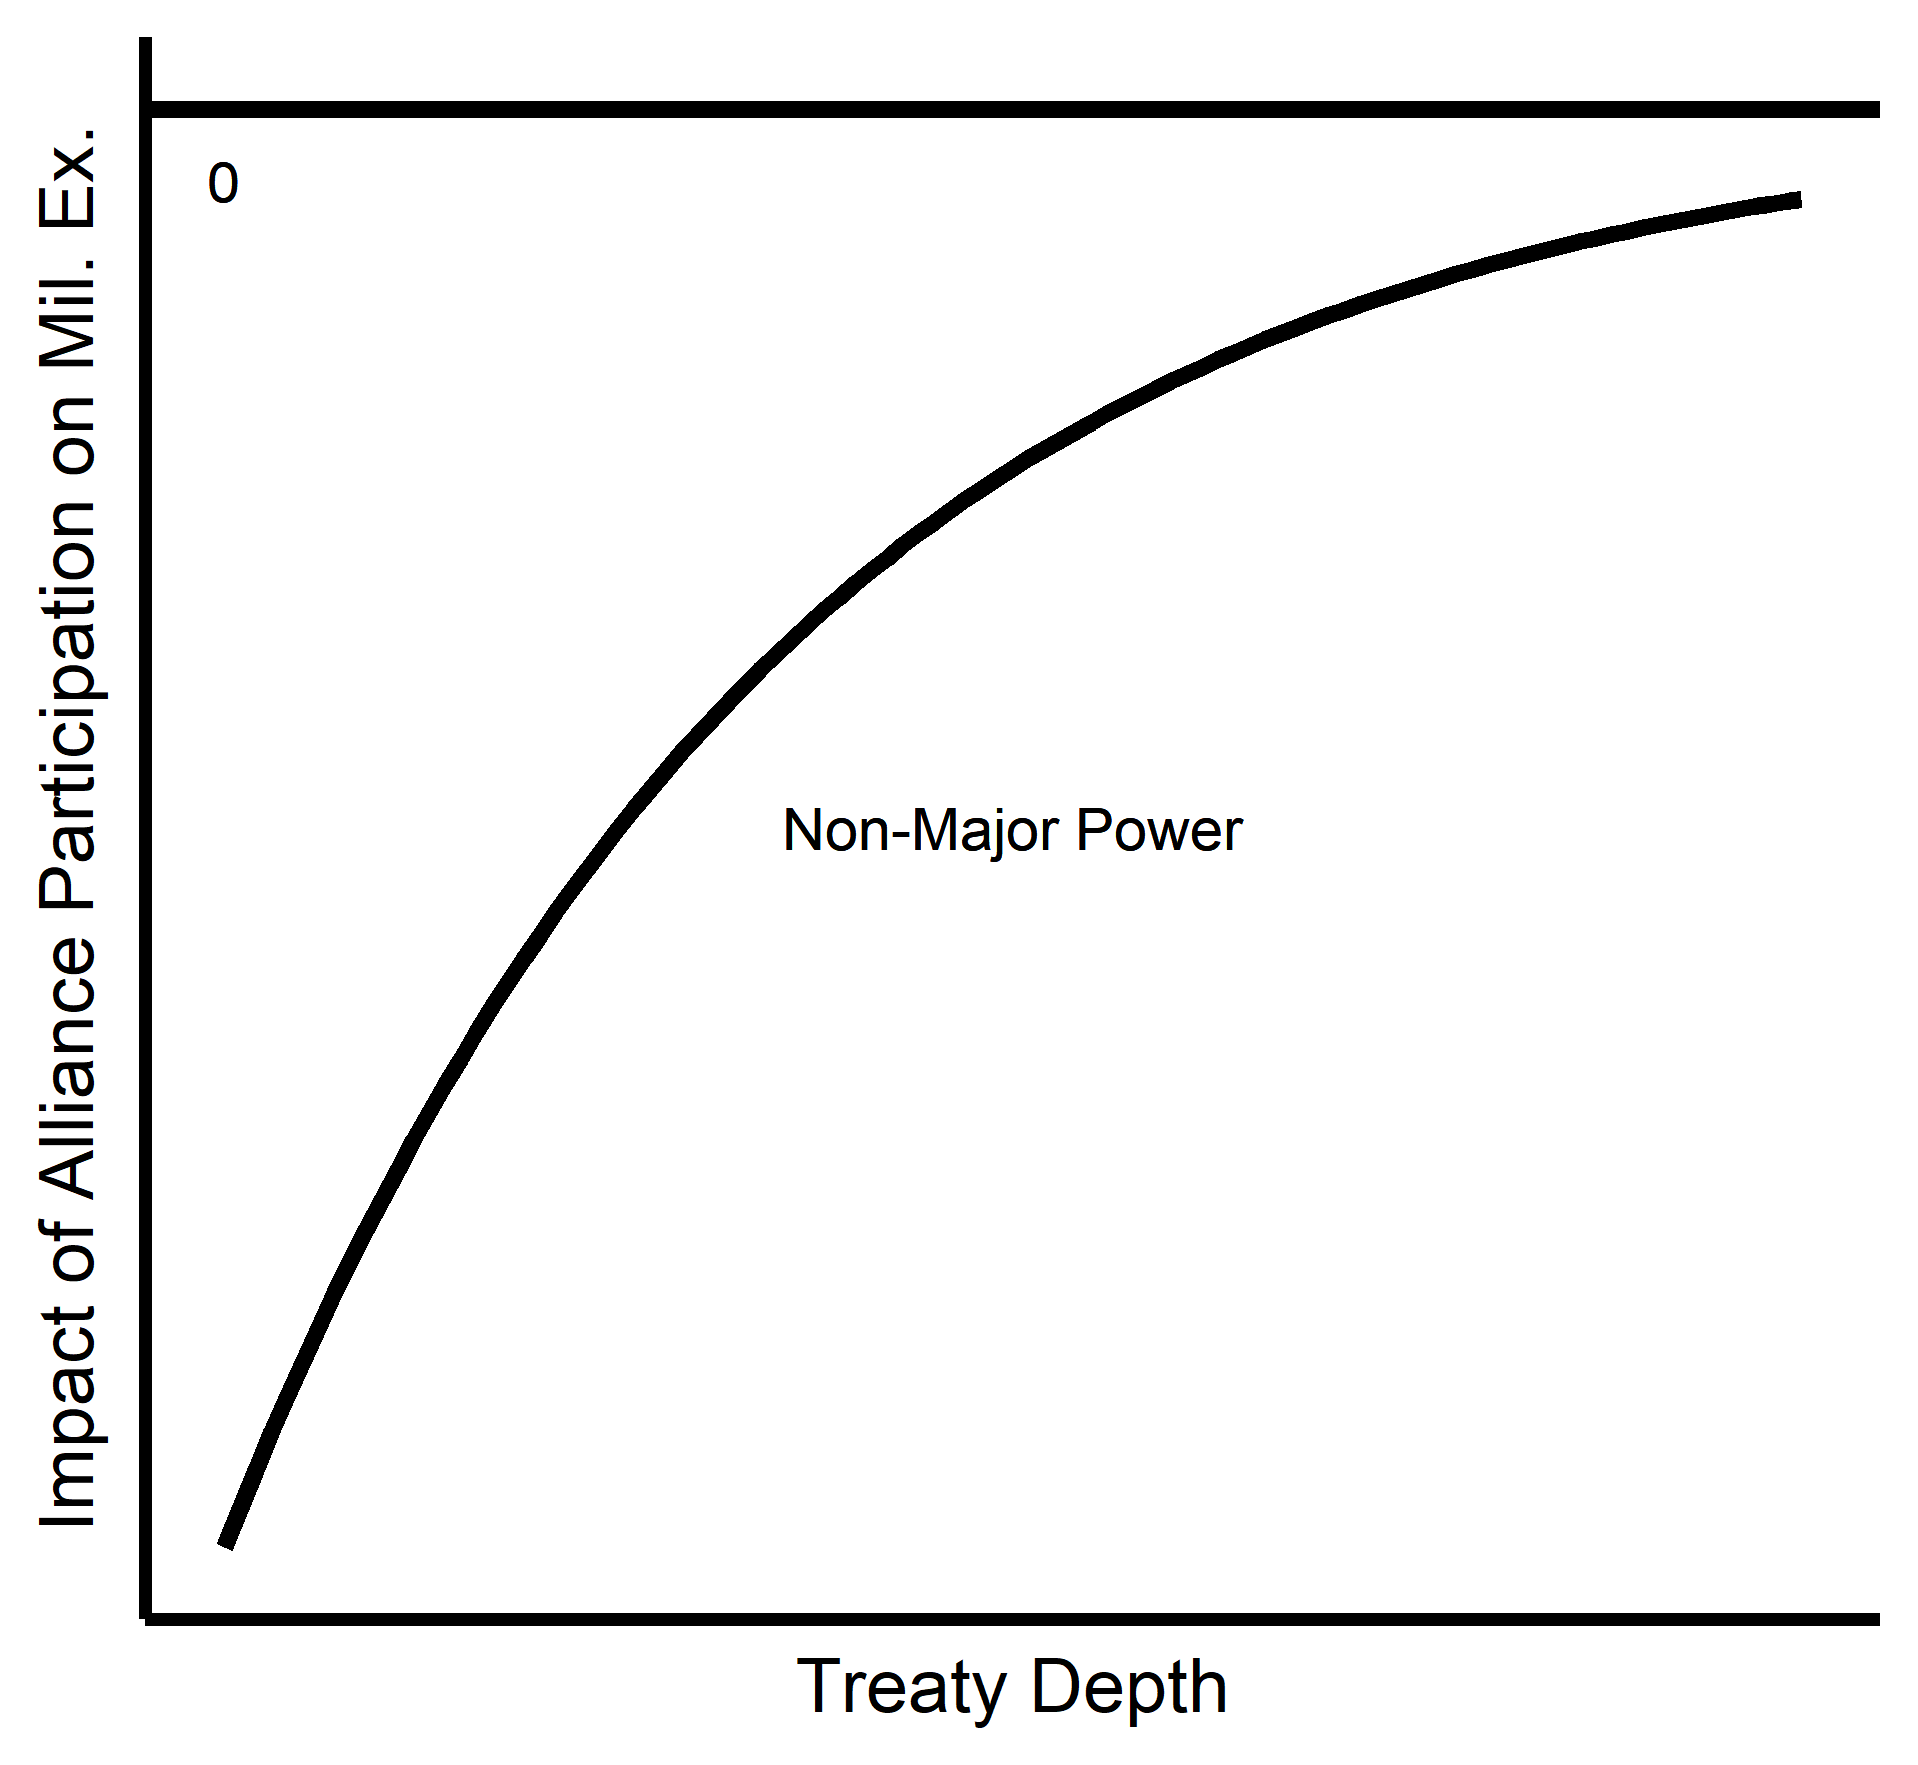
\includegraphics[width=0.95\textwidth]{../figures/illus-arg.png}
	\caption{Abstract illustration of the link between treaty scope and the impact of alliance participation on military spending.
	The top curve represents changes in the impact of alliance participation on growth in major power military spending as treaty scope increases.
	The bottom curve plots the same function for non-major powers.}
	\label{fig:illus-arg}
\end{figure}


\autoref{fig:illus-arg} illustrates my claims about military spending by plotting a hypothetical link between treaty scope and the impact of alliance participation on military spending. 
I do not derive a formal function connecting scope scope and the impact of alliance participation, so this exact functional form is not essential to the argument.\footnote{However, the convexity and concavity of each function are plausible because alliance participation and military spending are imperfect substitutes.}  
Instead, \autoref{fig:illus-arg} shows the need to be careful moving between changes in spending growth and changes in levels. 


For major powers, lower military expenditure growth as treaty scope increases may still lead to higher spending levels. 
Greater treaty depth reduces the standard positive correlation between treaty participation and military spending for major powers. 
Even deep treaties may still increase growth in military spending, however. 
Under these circumstances, lower growth in spending from greater treaty scope will not reduce the observed level of major power military spending. 


For non-major powers, increasing growth in spending from expanding treaty scope may still result in lower expenditure levels. 
Deeper treaties attenuate the usual negative correlation between alliance participation and military spending in non-major powers. 
But so long as the cumulative impact of alliance participation is negative, the observed level of military spending will fall. 


Of course, some treaties may lead to increases in non-major power military spending because the impact of alliance participation on military spending depends on more than treaty scope. 
Other alliances could reduce the level of major power military spending through negative spending growth.
Thus, this figure is incomplete, but it is a useful illustration of my claims about treaty scope. 


The argument proceeds as follows.
First, I describe key characteristics of states and the actions they take for foreign policy gain. 
Then I describe a general framework to understand alliances and summarize the sources and implications of alliance treaty scope. 
Last I connect alliance formation and maintenance to growth in military spending for major and non-major powers, and detail the consequences of differences in treaty scope.  



\subsection{States and Alliances}


% States are the actors: value FP good and domestic consumption  
My argument focuses on the behavior of states. 
I assume states value both domestic consumption and foreign policy goods \citep{Powell1993, Fearon2018}. 
The two major foreign policy goods are security and influence. 


Security is the freedom to hold territory and consume wealth as a state sees fit. 
Influence is the ability of a state to shape international relations in beneficial ways. 
While security is essential, influence is more of a luxury good. 
To secure these foreign policy goods, states can increase their military capability through military spending or join alliances. 
Alliances and military spending have different costs. 


% assumptions about world (1): opp costs of milex
I assume growth in military spending has domestic political opportunity costs--- funds spent on the military cannot be used for other goods. 
Greater military spending reduces domestic consumption \citep{Fearon2018}. 
These opportunity costs are decreasing in state size, however. 


Larger states have a lower tax price of spending, and benefit from economies of scale. 
As the number of taxpayers falls, the marginal cost per taxpayer of an increase in military spending rises \citep{DudleyMontmarquette1981}. 
This greater tax price reduces demand for military spending. 
For economies of scale, producing more defense goods lowers the cost of additional units \citep{Moravcsik1991, AlesinaSpolaore2006}. 
Thus, larger and more capable states have lower opportunity costs of military spending. 


% assume (2): alliances- leads to general framework to understand alliances
I also assume alliances are a costly signal of shared foreign policy interests. 
Alliances promise military support in the event of conflict. 
The formal hands-tying signal in a treaty generates a credible commitment to intervene \citep{Fearon1997, Leeds2003}.
Alliance members give up some freedom of action by tying their hands, which increases their security or influence. 


% Two stages, formation and maintenance (could say continuation) 
Alliance participation includes formation and maintenance \citep{Snyder1997}. 
During formation, prospective members determine what arrangement will provide the foreign policy benefits they seek at an acceptable cost. 
Formation produces the initial foreign policy gains and restraints on freedom of action. 


After a treaty forms, members must maintain their alliance in the face of a time inconsistency problem. 
Alliance formation reflects shared foreign policy interests, but interests change over time. 
Diverging interests increase the risk of opportunistic behavior by allies \citep{Leeds2003a, LeedsSavun2007}
Changing interests over time generate demand for reassurance that members are committed to upholding their promises. 


Reassurance requires additional costly signals. 
Maintaining or increasing military spending, aid, or cooperation on other issues are all costly signals of commitment. 
Bearing these costs indicates ongoing commitment to the treaty. 
On the other hand, failure to signal commitment will undermine the alliance. 


% contracting.
Because alliance formation and maintenance are costly, members bargain over the distribution of costs and benefits.
States design alliance treaties to address this distributional problem and potential opportunistic behavior. 
Therefore, observed treaty content reflects a mutually acceptable division of benefits and costs. 
Alliances can be thought of as a contract where states design alliance treaties to addresses opportunism and distributional problems \citep{Williamson1985, Koremenosetal2001} so members can realize gains from exchange \citep{Lake1996, Bensonetal2014}.


% treaty heterogeneity- product of design 
In specifying an alliance contract, states employ a wide range of formal promises. 
Design choices impose costs on members and shape the benefits they receive.
Because states form treaties they intend to honor, treaty content provides information to members and potential adversaries \citep{Leeds2003}. 
Members and adversaries can use formal promises to predict if a treaty will be honored.


When a treaty contains many costly promises, observers can infer the commitment is more credible. 
Additional credibility is valuable, because not all alliances are equally credible \citep{Benson2012}. 
The formal scope of commitment is therefore a crucial difference between treaties.\footnote{I use treaty scope as shorthand for the costliness and depth of formal promises in an alliance treaty.} 


% chaning treaty scope shapes the consequences of alliance participation 
Changes in treaty scope alter the consequences of alliance participation for growth in military spending among member states. 
I assume alliance treaties have heterogeneous effects on military expenditures and use treaty scope to explain those differences. 
Membership in a deeper treaty has different consequences for military spending than membership in a limited treaty. 


\subsection{Treaty Scope}


% diff costs and credibility
What determines the formal scope of an alliance treaty? 
Deep commitments stipulate deep and costly cooperation among members.
Allies incur higher costs from adding extra promises to core obligations of military support and risk more consequences from breaking such a treaty. 


Some treaties focus on promises of military support. 
These alliances make the minimum possible commitment. 
However, promises of military support are still valuable, because these define the essential scope of the alliance.  
Conditions on military commitments further define the scope of the treaty. 


% promises of support & costs of violation 
Not all alliances provide clear promises of military support--- some are limited to non-aggression, neutrality or consultation. 
Commitments to fight expose states to the risk of bearing the costs of war on behalf of their ally. 
When an alliance is invoked, violating the treaty is also costly. 
Backing out of a promise to fight has audience \citep{Levyetal2015} and reputation costs \citep{Gibler2008, Crescenzietal2012, Mattes2012}. 
So promises of military support expose states either to risk of fighting, or bearing the costs of treaty abrogation. 


Unconditional promises of military support increase the scope of an alliance. 
An unconditional commitment promises intervention no matter how or where the conflict began. 
Placing no conditions on intervention expands the scope of military support, but it creates other issues. 
Once a treaty is invoked, unlimited promises of support can either be violated or honored--- there is no way to disavow the obligation. 
This can expose states to entrapment in unwanted conflicts \citep{Snyder1990, Benson2012}, or the costs of violation. 
Simply put, placing few conditions on military support increases the set of circumstances where the treaty applies.  


% sunk costs commitments
States can add further scope to their alliances by tying other costly commitments to the central promise of military support. 
States incur the costs from these promises during treaty formation and often continue to bear them to maintain the alliance.\footnote{
One salient cost applies to all treaties--- backing a partner precludes alliances with potential antagonists \citep{Snyder1997}.} 
These sunk cost promises include aid, economic concessions, integrated military command, basing rights, international organization formation and concluding other agreements. 


All of these commitments add scope to the alliance by expanding ties among partners. 
Sunk cost promises create a web of additional obligations which reinforce the core promise of military support.  
For example, granting economic concessions shows a state is willing to bear costs to support an alliance \citep{WolfordKim2017}. 


% Gain more from an alliance
Treaties with greater scope are more credible \citep{Poast2013}. 
Making sunk cost commitments and potentially costly promises of military support increases the credibility of deep formal treaties.
That credibility produces more foreign policy benefits for members. 
But foreign policy gains come at the cost of reduced freedom of action. 


% Tradeoff: credibility vs freedom of action 
Greater treaty credibility is the result of members limiting their ability to behave opportunistically. 
In a credible treaty, there is less doubt a state will honor its alliance commitments, which implies that partners have ruled out other potential actions. 
Restricting the set of possible choices and making some actions more costly reduces alliance members' freedom of action. 
Forming an alliance makes nonintervention more costly, rules out alternative treaties and requires coordination among members \citep{Snyder1997}. 


All states face a tradeoff between treaty credibility and freedom of action. 
The promises that make a treaty more credible also constrain participants. 
States manage this trade-off through treaty design. 
Greater treaty scope reflects a willingness to accept lost freedom of action for greater freedom of action. 
The implications of this tradeoff for growth in military spending depend on state capability. 


% diff consequences due to heterogeneity among states 
State capability shapes what foreign policy goods states pursue with their alliances. 
Less capable states focus on territorial security through military spending and alliances. 
More capable states use alliances and military spending to expand their influence in international relations. 
While many states focus on immediate security, others invest in extra capability to pursue more ambitious foreign policy goals \citep{Fordham2011, MarkowitzFariss2017}. 


\subsection{Major Powers} 


% seeking influence abroad
Major powers are the most capable and ambitious actors in the international system. 
These states have a wide range of foreign policy interests due to their economic ties, size, and ability to pursue a wide range of issues. 
Given their capability and interests, major powers pursue goals beyond their immediate security. 
Major powers seek influence--- reshaping international relations to match their interests by changing the behavior of other states. 


% influence from arms and allies: balance entanglement and influence 
Influence comes from changing the expected outcome of conflicts between other states.
Altering the value of international conflict shifts how major power proteges and adversaries behave.  
How much influence a major power has depends on how likely they are to intervene and their military capabilities. 
Expressed as an abstract equation, influence is a product of the likelihood of intervention and capability: $\mbox{Influence} = \mbox{Change War Outcome} = \mbox{Probability of Intervention} \times \mbox{Capability}$.


% Mix of both alliances and arms
Therefore, military spending and alliances are both sources of influence. 
Alliances increase the probability of intervention. 
Military spending adds capability, making a potential intervention more effective. 
In general, major powers will use a mix of greater alliance participation and military spending to realize desired changes in their influence. 


% Increasing size reduces the opportunity costs of defense spending
Major powers are willing to increase alliances and military spending simultaneously due to their lower opportunity cost of defense spending. 
Greater economic size and capability reduces the tax price of spending and generates economies of scale. 
As a result, major powers have the capacity to expand their defense budget in pursuit of influence.  


Additional military spending supports alliance commitments, while alliances make promises to use that capability more credible. 
Therefore, major power alliance participation will often lead to increasing growth in spending. 
Supporting an alliance by growing military spending is worthwhile because treaties give influence through exchange. 


% think about formation: influence vs entanglement
Major powers provide military support in exchange for influence over their partner. 
This exchange is obvious in asymmetric treaties between major and non-major powers \citep{Morrow1991}. 
In return for protection, junior partners surrender some autonomy \citep{Lake2009}. 


% Expand on symmetric treaties- less obvious
Symmetric alliances with other major powers are also a source of influence through exchange.
The most capable states can lose territory in war, but defeat is rarely an existential threat \citep{Fazal2011}.  
Major power partners in symmetric treaties secure their territory, but these treaties are more focused on reshaping international relations. 


Alliances between major powers clarify otherwise implicit alignments, giving partners greater leverage. 
Clarifying alignment defines potential spheres of influence and creates expectations of support on other issues \citep{Snyder1997}. 
In exchange for military support, states settle outstanding issues, or promise support elsewhere. 
Major power alliances often delineate territorial or colonial divisions \cite{Langer1950, Kissinger1994}.
For example, the 1904 Entente Cordiale between France and Britain included ``a systematic effort to settle all outstanding colonial issues'' \citep[pg. 189]{Kissinger1994}.   


% here's the entanglement
These symmetric and asymmetric treaties come with the cost of greater involvement abroad.
Major powers must engage more to manage alliance partners and maintain commitments.
These ``foreign entanglements'' build influence but constrain freedom of action.
Alliance treaty design tackles this tradeoff between influence and entanglement. 


% treaty design to manage tradeoff
Major powers balance entanglement and influence by adjusting the scope of their formal commitments. 
Deeper alliance treaties increase both influence and entanglement. 
A broad formal commitment is more credible, but also stipulates deeper engagement abroad. 
Less credible treaties are more ``arms length,'' which allows major powers to retain more freedom of action. 


When major powers prioritize influence through alliances, they will make deeper formal commitments.
But when they fear entanglement abroad, they will make limited formal treaties. 
Once a treaty forms, the depth of a formal commitment alters how major powers maintain the alliance. 


% think about maintenance- leverage over partners and need to uphold treaty 
Alliance maintenance by major powers must address allied fears of abandonment and distorted incentives. 
Because major powers provide large amounts of capability, abandonment has huge consequences for partners. 
Imagine if the US did not support Lithuania after a Russian attack, for example. 
Thus, partners need assurances the major power will not abrogate the treaty. 


Growing military spending is one way for major powers to reassure their allies--- it signals a willingness to support their commitments. 
Opportunity costs make ongoing investments in military capability a credible signal of commitment, but these investments distort allied incentives \citep{Lake1996, Lake2009}. 
Given the opportunity, allied states can reduce military spending and rely on more capable partners for protection.
Lower allied defense expenditures leaves major powers to bear a greater burden if war breaks out. 


The tension between reassurance and distorted incentives generates a challenge for major powers--- they must reassure their allies without bearing excessive costs.
Too much reassurance allows partners to reduce defense expenditures, placing more of the burden of providing capability on major powers. 
Inadequate reassurance leads allies to question the credibility of the alliance itself, jeopardizing influence.   
There are other ways major powers can reassure their allies and check distorted incentives. 


Threatening to abandon the treaty entirely is a possible check on reduced defense spending by allied states. 
But so long as foreign policy gains from a treaty outweigh maintenance costs, major powers cannot credibly threaten to abandon free-riding allies. 
Abandonment is only credible when foreign policy interests have changed dramatically, or the costs of maintaining a treaty are astronomical. 


If threats of abandonment rarely provide leverage in alliance bargaining, how else can major powers avoid bearing excessive costs? 
Increasing the scope of formal treaty commitments provides other ways to maintain a treaty.
Sunk costs provisions make a treaty more credible and provide ongoing reassurance.
By continuing to provide side payments, major powers signal continued commitment. 

 
Forming a deep alliance with multiple costly promises then gives major powers more leverage over partners. 
Instead of threatening to abandon the treaty, they can bargain using other issues. 
Major powers can condition maintaining aid, economic agreements or integrated military command on adequate defense effort.
This bargaining establishes issue linkages between treaty commitments and allied contributions. 


Ongoing issue linkages are viable because most sunk costs promises incorporate repeated transfers, not one-shot infusions. 
Failing to make promised payments imposes costs on allies without destroying the treaty. 
Providing side-payments and bundling them with military support can also offset the costs of greater defense effort for allies. 


% connect with treaty scope 
A deep formal treaty with costly promises of military support and sunk costs commitments is therefore a greater source of influence.
Greater influence comes from increased credibility in the treaty and greater bargaining leverage with allies.  
By forming a deep treaty, major powers gain more influence without as much growth in military expenditures. 
A limited treaty would require more spending to reach the same level of influence. 
Therefore, greater treaty scope substitutes for growth in major power military spending. 


Britain's alliances in the Middle East after World War II illustrate how major powers can offer deep treaties as a substitute for investment in military capability. 
After World War II, the UK faced acute economic challenges while attempting to maintain their influence in the Middle East. 
``In securing a victorious outcome to the war, the British had severely overstrained themselves'' \citep[pg. 367]{Kennedy1987}. 
To finance the war London ``liquidated over \textsterling1 billion of overseas investments and at the same time had brought the general foreign debt to more than \textsterling3 billion'' \citep[pg. 12]{Louis1984}.
 

Even so, the UK attempted to maintain an expansive foreign policy \citep{Mayhew1950}, especially in the Middle East \citep{Rahman1982}. 
But troop deployments were a major economic burden. 
Winston Churchill attacked the Labour government because ``nearly 100,000 British soldiers had been kept in Palestine, and \textsterling30,000,000 or \textsterling40,000,000 a year of our hard-earned money had been cast away there.''
\footnote{Quoted in \citet[pg. 11]{Louis1984}.}
Therefore, the government was unwilling `` to endorse political or economic settlements that might have required British bayonets'' \citep[pg. 15]{Louis1984}. 


Because economic factors constrained military spending, the UK looked for other ways to uphold their influence \citep{Monroe1963, Louis1984}
London created deep alliances with Jordan (ATOPID 3125), Libya (ATOPID 3235) and Iraq (ATOPID 3280).\footnote{Negotiations with Egypt were undone by Arab nationalism and the rise of Nasser.} 
In return for basing rights, Britain promised aid, committed to defense consultations, and promised to resolve disputes through the International Court of Justice \citep{Leedsetal2002}. 
These commitments added greater scope to promises of military support. 
Before World War II, London exerted influence through a preponderance of capability \citep{Monroe1963}.
After World War II, the UK increased the scope of their alliance treaties to maintain influence in the Middle East without spending as much on the military. 


My argument and the British case suggest that greater treaty scope will reduce the tendency of alliance participation to increase growth in major power military spending.
Consider a hypothetical major power choosing between a deep and shallow formal treaty to achieve a particular level of influence.  
Most treaties require growth in spending, but a deeper treaty provides equivalent influence with less growth in defense expenditures. 
Therefore, growth in major power military spending from alliance participation will be positive and decreasing in treaty scope. 


% Prediction (H1 right here) 
\begin{quote}
\textsc{Hypothesis 1}: As alliance treaty scope increases, growth in major power military spending will decrease. 
\end{quote}


To be clear, I do not claim that greater treaty scope will lower the \textit{observed level} of major power military spending. 
Lower growth in spending, especially when alliance participation generally leads to increasing defense spending, need not reduce the size of the defense budget. 
The level of spending may be lower than some counterfactual scenario with a limited treaty, but the observed level probably will not fall. 


The logic of treaty scope and major powers also suggests that even relatively shallow treaties should lower growth in major power defense spending. 
Achieving greater influence without alliances requires massive growth in military expenditures. 
A limited alliance still provides more foreign policy gains than no treaty at all. 


The logic behind Hypothesis 1 does not apply to non-major powers. 
These states have different goals and constraints. 


\subsection{Non-Major Powers} 


% Non-major powers focus on security
Non-major powers seek immediate security by using alliances and military spending to protect their homeland.  
In doing so, they have greater opportunity costs of military spending. 
Limited economies of scale in defense and a higher tax price of military spending increase the marginal costs of military expenditures for non-major powers. 
Growth in military spending is a more serious constraint on domestic consumption in these states, all else equal.
\footnote{Economic growth diminishes this tradeoff.} 
As a result, non-major powers have strong inducements to reduce growth in defense spending whenever possible.


Relying on allies is one way for non-major powers to maintain their security and lower growth in military expenditures.  
Allied protection provides additional security without requiring more military spending. 
Alliance participation will generally reduce growth in non-major power military spending. 
Even so, alliance participation does not always lower expenditure growth.
 


% Intro tradeoff 
Though deeper formal treaties provide more security, they also limit the freedom of non-major powers to reduce growth in defense spending.
Greater credibility makes deep treaties a valuable source of security. 
Lost freedom of action in these alliances is the result of greater treaty value and increased allied influence. 
Therefore, non-major powers must balance security and freedom of action in alliance formation. 


% think about formation- security vs freedom to reduce opp costs of milex
Alliance treaty design will reflect the relative value non-major powers place on security and freedom to set military expenditures. 
When security is more important, non-major powers will accept lost freedom of action in a deep formal treaty.
When these states prioritize domestic consumption, shallow commitments will prevail. 
Alliance maintenance reinforces this tradeoff between security and domestic consumption. 


% think about maintenance- influence of partners and need to uphold treaty
Like major powers, non-major powers maintain alliances by signaling ongoing commitment as interests change. 
Higher growth in military spending is a costly signal of commitment for major powers, because it has substantial opportunity costs. 
Maintaining adequate military capability also helps avoid antagonizing partners. 
If non-major powers fail to invest enough in military capability, they risk undermining the treaty by shifting too much of the burden of fighting to partners. 
Adding to allied costs of maintaining the treaty could lead to abandonment. 


As treaty scope rises, non-major powers have extra inducements to signal commitment by allocating resources to the military.
First, deep treaties are more valuable, increasing the downsides of undermining the treaty. 
Signaling commitment ensures continued access to valuable side payments.   
Because deeper treaties give more security, non-major powers are more willing to bear the opportunity costs of military spending. 
Additional security offsets the opportunity costs of military spending under these treaties.
Other constraints are less voluntary.   


Deeper ties give allies influence to demand additional defense spending. 
I have already argued major powers can use issue linkages to bargain about defense spending. 
This influence extends to more coercive bargaining that uses side payments from formal alliance promises as leverage. 
Reducing growth in military spending is more costly if allies withhold aid or economic concessions. 


As the number of sunk costs commitments falls, allied leverage declines. 
Without side payments, allies are reduced to threatening to leave the treaty unless allied expenditures pick up. 
But these threats are rarely credible, because abandoning a treaty eliminates the benefits of participation. 


In a shallow treaty, non-major powers have more freedom of action.  
These agreements provide less security.  
Even so, limited treaties still provide security--- a limited alliance is better than no alliance at all. 


As a result, non-major powers will reduce growth in military spending under shallow treaties. 
But as treaty scope rises and constrains non-major powers' freedom of action, growth in military spending will rise. 
Limited commitments provide security and enough freedom of action for non-major powers to lower growth in military spending and expand domestic consumption. 
Greater treaty scope increases treaty value and allied influence, increasing growth in military expenditures. 


% Prediction (H2 here) 
\begin{quote}
\textsc{Hypothesis 2}: As alliance treaty scope increases, growth in non-major power military spending will increase. 
\end{quote}


% Transition para
My argument focuses on differences between deep and shallow treaties, so the research design must compare treaties and measure alliance treaty scope.  
I use a measurement model to infer treaty scope from formal content, then connect alliances to state military spending with a multilevel model. 
The next section describes the research design in more detail. 



\section{Research Design} 


% two contributions: Develop latent str. measure and then put it into an ML model
My research design makes two contributions. 
First, I develop a latent measure of alliance treaty scope. 
Then I employ that measure in a multilevel model, connecting alliance-level variation with state-level outcomes. 
The multilevel model bridges specific and general research designs by simultaneously estimating the specific impact of each alliance on military spending and the general impact of different alliance characteristics. 
To examine differences between major and non-major powers, I estimate the multilevel model in separate samples of major and non-major powers from 1816 to 2007. 
The next section describes my measure of alliance treaty scope. 


\subsection{Measuring Alliance treaty scope} 


% Intuituion behind latent measures: observed char reflects underlying concept
My argument implies observed alliance promises reflect the underlying scope of the treaty. 
Deeper alliance treaties will contain more costly promises. 
Therefore, I use observed alliance characteristics to infer treaty scope.


Treaty scope depends on the potential costs of core support, and supplementary sunk cost promises in the pact. 
The potential costs are tied to core commitments of defensive or offensive military support, and conditions on support.\footnote{Some alliances promise only neutrality, consultation, or non-aggression, rather than military support.}  
Sunk costs promises in alliances include integrated military command, forming international organizations, basing rights, promises to make other agreements, and economic or military aid. 
All of these commitments are theoretically relevant, so the measure must incorporate multiple observable indicators of strength. 


Conceptualizing observed treaty conditions as indicators of underlying scope could produce two measures. 
The first is constructing an additive index of treaty scope. 
Treaties with multiple costly promises would score higher on such an index. 
This assumes each indicator is equally important, which is unlikely. 
Instead, I employ latent variable modeling, which is a less restrictive way to use observable characteristics to infer an underlying trait. 


Latent variable modeling offers a flexible and intuitive way to measure alliance treaty scope. 
My argument expects that there is a single factor underlying variation in potential and sunk costs across treaties.  
The measurement model estimates the correlations between alliance treaty content and the underlying formal scope, and then infers the likely values of strength. 


% Justify use
Measurement models have a rich history in political science and have produced notable measures of ideology \citep{Clintonetal2004}, democracy \citep{TreierJackman2008} and human rights \citep{Fariss2014}. 
\citet{BensonClinton2016} use the mixed factor analysis model of \citet{Quinn2004} to measure alliance scope, depth and capability.
I emulate Benson and Clinton's approach, but employ more indicators of scope and a different estimator. 


% How the model works
I use the Bayesian Gaussian Copula Factor Model of \citet{Murrayetal2013} to generate a measure of alliance treaty scope. 
Murray et al's model improves mixed factor analysis for continuous, ordinal, and binary observed data by relaxing distributional assumptions. 
Given discrete observed variables and non-Gaussian latent variables, the dependence among the latent variables and their marginal distributions are both influenced by the latent variables.
Their model encodes the dependence structure of multivariate latent data using a copula
\footnote{Copulas are distribution function on $[0, 1]^p$ where each univariate marginal distribution is uniform on $[0,1]$. This function encodes the dependence structure of a multivariate distribution.} 
and expresses the latent variables and factor loadings as a series of latent normal variables. 
The semiparametric approach breaks the dependence between the latent factors and marginal distributions, improving inferences about the latent variable. 


Besides its semiparametric component, this measurement model employs a general factor analytic approach.
Factor analysis estimates the association between observed variables and some latent factor.
Each observed variable has a factor loading--- the association between the observed variable and the latent variable.  
Like standardized regression coefficients, factor loadings range from -1 to 1, so observed variables are positively or negatively correlated with the latent factor.  


For each observation, a linear combination of observed alliance characteristics predicts latent treaty scope, like a regression with an unobserved outcome.  
I estimated the model using observed data from all 745 alliances in the alliance-level ATOP data \citep{Leedsetal2002}. 
Indicators of treaty scope are divided between the potential costs of abrogation and sunk costs commitments.
The potential costs depend on promises of defensive support, offensive support, neutrality, consultation, non-aggression and unconditional military support. 
Sunk costs include military aid, economic aid, bases, international organization formation, integrated military command, as well as promises to form new agreements in multiple issue areas and to forgo competing alliances. 
The theoretical argument suggests there is one latent factor underlying variation in all 13 indicators, so I fit the model with one latent factor. 


I used Parameter expanded Gibbs sampling, the default generalized double Pareto (GDP) prior, 10,000 burn-in iterations of the MCMC chain, and 20,000 samples thinned every 20 observations to ensure convergence. 
The resulting estimates include posterior distributions for the factor loadings and the latent factor. 
Because treaty scope is the main quantity of interest here, I focus on the posterior distributions of the latent factor. 


% Show the measure for all alliances- note I'll only focus on treaties w/ military support.
Each alliance has a unique posterior distribution of its latent scope. 
I use the mean of that posterior to measure treaty scope--- the mean is the expected scope of a treaty, given its content. 
\autoref{fig:ls-summary} describes the latent measure for ATOP alliances  with military support from 1815 to 2016.
I focus on the 289 treaties offering military support because prior studies of alliance participation and military spending emphasize these treaties.\footnote{
I estimated the measurement model on all alliances to capture the contributions of defensive and offensive conditions to treaty scope.}
Each alliance has a unique scope score, so my measure contains the expected strength of an alliance treaty, conditional on the formal promises it makes. 


There is substantial variation in the scope of alliance treaties. 
The top panel of \autoref{fig:ls-summary} is a histogram of mean treaty scope for alliances promising military support. 
Variation between these treaties is driven by sunk costs promises and conditions on military support. 
Most treaties are concentrated between .5 and 1.5 on the latent scale, but approximately 40 treaties are deeper or shallower. 
The bottom panel of \autoref{fig:ls-summary} plots the posterior means and uncertainty in those estimates against the start year of the treaty. 
Even after accounting for posterior uncertainty, it is possible to distinguish between treaty commitments. 


\begin{figure}
	\centering
		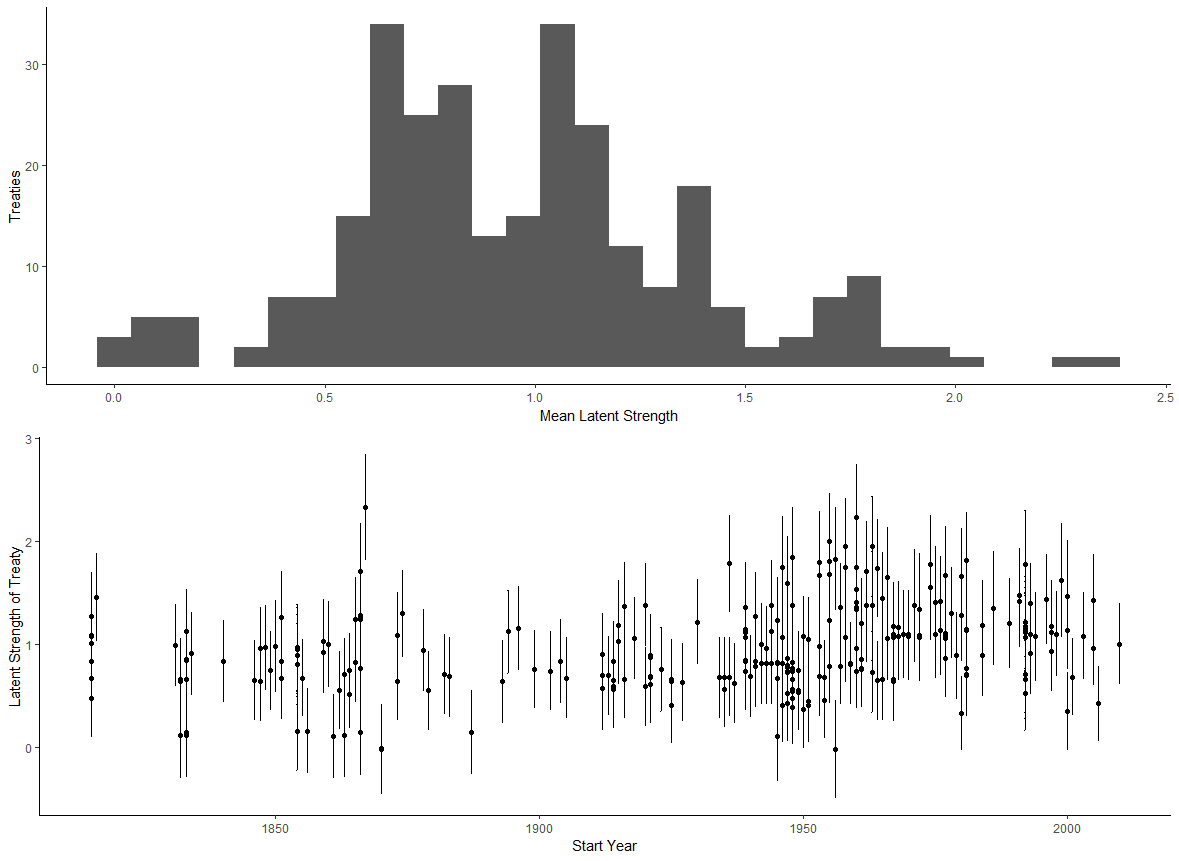
\includegraphics[width=0.95\textwidth]{../figures/ls-summary.png}
	\caption{Summary of latent measure of alliance treaty scope for 289 alliances promising military support from 1816 to 2016. The top panel is a histogram of the expected of alliance treaty scope. The bottom panel plots mean treaty scope (points) and the standard deviation (error bars) against the start year of the treaty.}
	\label{fig:ls-summary}
\end{figure}


% Cases- especially deep and shallow treaties
The measure makes clear distinctions between treaties. 
Although the values of the latent measure are not intrinsically informative, differences between treaties on the latent scope scale are meaningful. 
Thus, I can make comparisons between treaties based on their latent measure scores. 
The mean of treaty scope is 0.92, and the median is 0.90. 
The median treaty is an 1854 agreement between Austria, France, and Britain against Russia in the Crimean war (ATOP ID 1180). 


The most limited treaty is an 1870 neutrality and offense pact between France and Britain (ATOPID 1300), which Britain used to protect Belgian neutrality during the Franco-Prussian war.  
Britain formed an identical alliance with Prussia in 1870, which scores nearly the same on the latent measure.\footnote{
Sampling variation means the scores will not be exactly the same.} 
Both treaties have only offensive and neutrality promises, conditional on France and Prussia respecting Belgian neutrality. 
Otherwise, the UK made no sunk costs promises, so these two alliances are as limited as possible. 


NATO (ATOPID 3180) has a mean latent scope score of 0.73, placing it in the second quartile of military support alliances. 
NATO's two costly provisions are the defense obligations in Article 5 and establishing the Atlantic Council. 
According to the ATOP coding sheet for NATO, ``There are numerous bilateral agreements among NATO members re: military aid, bases, etc. but they do not qualify as separate alliances, nor are they part of the overall NATO structure.''
NATO treaty is below average in formal scope in part because additional costs were negotiated outside the formal treaty.    


The three deepest treaties are an 1867 alliance between Prussia and Hesse (ATOPID 1290), a 1955 treaty between Greece, Turkey and Cyprus (ATOPID 3400) and the United Arab Republic (ATOPID 3300).  
All these treaties supplement promises of military support with costly promises of cooperation. 
The United Arab Republic attempted to unify Syria and Egypt, so it promises defense, integrated command, military aid, multiple international organizations, and basing rights. 
In the alliance between Greece, Turkey, and Cyprus, Greece and Turkey set up military aid, integrated military command, international organizations to mange relations on the island--- a limited commitment would have lacked any credibility. 
These extra costs made arrangements between historic enemies in Cyprus more credible. 
The UAR and Greco-Turkish treaties were undone by domestic coups, one in Turkey, the other in Syria, but that does not diminish the depth of cooperation they sought. 


The latent measure has some face, concept, and discriminant validity of the latent measure. 
For face validity, the UAR is a deeper and more costly commitment than a promise to respect Belgian neutrality. 
The most shallow treaties make few costly promises beyond military support, matching my conceptualization of treaty scope. 
Last, this measure can distinguish between deep and shallow commitments. 


My argument uses variation in treaty scope between alliances to explain growth in military spending.
Deep and shallow treaties should have different effects. 
While the independent variable is alliance-level scope, the outcome is state-year growth in military spending. 
Therefore I use a multilevel model to estimate the association between this measure of treaty scope and alliance members' military spending.  
The next section summarizes the multilevel model in more detail. 


\subsection{Multilevel Model} 


% Best fit for theoretical process. Can compare alliances. 
Multilevel modeling is a natural way to bridge levels of analysis, and it incorporates elements of the specific and general research designs in previous research. 
Specific studies focus on responses to allied spending in particular treaties, while general studies in panel data rely on coarse aggregates of alliance participation.
In this model, I estimate the specific impact of each alliance on members' military spending as well as the general association between treaty scope and military expenditures. 
I can simultaneously make inferences about the impact of individual treaties and the impact of treaty characteristics including strength. 
To facilitate computation and interpretation, I fit the multilevel model using Bayesian estimation in STAN \citep{Carpenteretal2016}.\footnote{See the appendix for details of the weakly informative prior distributions and evidence the chains converged.}


This strategy adds complexity to a more traditional panel data specification. 
But the additional components match the argument and data structure, while also generating novel inferences. 
Multilevel modeling connects the argument and research design. 
My predictions compare deep and shallow treaties, so an alliance level regression in this multilevel model contains the corresponding coefficient.
Relying on a state-level proxy for alliance strength generates different comparisons and reduces variation in the key independent variable.


Aggregating variables at a different level of analysis may produce misleading inferences \citep{McElreath2016}. 
Multilevel modeling retains the structure of the data, where states are members of multiple alliances. 
Connecting the alliance and state level of analysis then allows me to infer how alliance-level variation impacts annnual growth in state military expenditures. 


Besides connecting alliance and state level variation, the multilevel model generates novel comparisons between alliances. 
Specific studies can only compare a few treaties at a time, while general research designs aggregate multiple treaties into a single measure. 
The multilevel model estimates the unique impact of each alliance on members' military expenditures. 
Partial pooling of these alliance-specific parameters generates reasonable estimates for every treaty, which can then be used to compare treaties. 


In summary, multilevel modeling provides useful inferences about alliance participation and military spending. 
This model matches my argument that treaty scope modifies the impact of alliance participation on military spending. 
Furthermore, by estimating the cumulative impact of participation in each alliance treaty, the model generates new evidence to help test my predictions. 
The next section summarizes the model specification. 
 


\subsubsection{Model Specification} 

% Two separate but connected regressions
% State-level regression- alliances enter through spending matrix.
This multilevel model connects two distinct regressions. 
The base is a state-year-level regression, which is similar to a random effects panel data regression.
A second alliance-level regression predicts parameters in the state-level regression, like an interaction. 


The state-level regression starts with a distribution for the outcome:
\begin{equation}
y \sim student_t(\mu, \nu, \sigma)
\end{equation}
 

$y$ is the dependent variable--- growth in military spending. 
I model spending growth using a t-distribution with degrees of freedom $\nu$ to address outliers.\footnote{I estimate $\nu$ directly.}
$\sigma$ is analogous to the error term in a frequentist regression--- this captures unexplained variation in spending growth.  
$\mu$, the mean of the outcome, depends on several covariates.
\begin{equation}
\mu = \alpha + \alpha^{st} + \alpha^{yr} +\textbf{W}_{n \times k} \gamma_{k \times 1}  + \textbf{Z}_{n \times a} \lambda_{a \times 1} 
\end{equation}


Growth in spending is a function of an overall intercept $\alpha$, state and year varying intercepts $\alpha^{st}$ and $\alpha^{yr}$ and a matrix of state-level control variables $\textbf{W}$.
These components comprise a standard random effects model. 
The $\textbf{Z} \lambda$ term incorporates alliance participation.


$\textbf{Z}$ is a matrix of state participation in alliances. 
Columns correspond to each of the $a$ alliances in the data, and rows to state-year observations. 
If a state is not part of an alliance, the corresponding cell of the matrix is zero.
If a state is part of an alliance in a given year, the matrix cell contains the log of total allied military spending.


I use total allied spending in the alliance participation matrix because more capable alliances provide extra benefits.
Increasing allied capability makes promises of military support more valuable \citep{Johnsonetal2015}.  
$\textbf{Z}$ encodes a quasi-spatial indicator of alliance participation for all $j$ alliances in the data. 
States can be members of multiple treaties at once, so observations are not neatly nested. 
This specification allows each alliance to have a unique impact on military spending, even when states participate in multiple treaties. 


$\lambda$ is a vector of parameters which estimate the impact of participation in specific alliances. 
Because the non-zero elements of $Z$ are allied spending, the $\lambda$ parameters capture alliance members' responsiveness to greater allied capability. 
Each alliance has a unique $\lambda$ and the $\lambda$ parameters have a common distribution. 
The shared distribution assumes alliances are similar but different in how they impact growth in military spending. 
I then use alliance treaty scope and other alliance characteristics to predict differences between treaties. 


% Alliance-level regression:
The second part of the multilevel model uses alliance characteristics to predict how allied spending is associated with growth in military spending. 
The $\lambda$ parameters are the dependent variable in an alliance-level regression.
Therefore the impact of an alliance on members military spending depnds on treaty characteristics including scope. 
I focus interpretation on this second-level regression, where: 

\begin{equation}
\lambda \sim N(\theta, \sigma_{all})
\end{equation} 
and 
\begin{equation}
\theta = \alpha_{all} + \beta_1 \mbox{treaty scope} + \textbf{X} \beta
\end{equation}


% Like an interaction between alliance and state-level factors 
In this alliance-level regression, $\textbf{X}$ is a matrix of alliance-level control variables and $\alpha_{all}$ is the constant.
Adding $\sigma_{all}$ means predictions of $\lambda$ are not deterministic--- the alliance level regression contains an error term. 
The second-level regression includes treaty scope, and each $\beta$ parameter modifies the impact of alliance participation on growth in military spending. 
The $\beta$ parameters are like marginal effects in an interaction. 


Treaty scope is connected to military spending by changing the consequences of alliance participation.
This is an indirect link, but the indirect connection matches my argument that scope alters the usual impact of alliance participation on military spending.  
A change in treaty scope modifies $\lambda$, which alters growth in military spending.
Hypothesis 1 predicts $\beta_1$ will be negative among major powers, and Hypothesis 2 expects $\beta_1$ will be positive for non-major powers.  


% Provide an example observation
Consider one observation as an example of how the model works. 
Growth in Argentina's military spending in 1955 depends on Argentina's economic growth, political regime, conflict participation, and rival military spending. 
Argentine participation in the Rio Pact and OAS also changes growth in spending through allied capability. 


\begin{equation}
\begin{split}
& \mbox{Argentina 1955} = \mbox{Overall mean}
+ \mbox{Argentine Intercept} + \mbox{1955 Intercept} 
+ \mbox{Argentine Characteristics} \\
& + \lambda_{OAS} * \mbox{OAS Expenditure} + \lambda_{Rio} * \mbox{Rio Pact Expenditure}
\end{split} 
\end{equation}


$\lambda_{OAS}$ and $\lambda_{Rio}$ are a function of the alliance level regression. 
The institutional design and membership of these treaties alter the $\lambda$ parameter.
Other alliances have no impact on growth in Argentine military spending. 


In this model, the $\beta$ parameters capture the general association between key alliance characteristics and military spending. 
The $\lambda$ parameters express the total impact of participation in each alliance and heterogeneous effects of different treaties. 
Using alliance characteristics to modify the impact of alliance participation matches my conditional argument. 
I now describe the sample and covariates in the analysis.  



\subsection{Sample and Covariates} 

% Sample of states 
I estimate this model on two samples of states from 1816 to 2007--- one sample of major powers, the other of non-major powers. 
Splitting the sample means I cannot directly compare estimates from the major and non-major power samples, but it will show different trends in the two samples. 
A split sample followed by graphical comparison of the estimates is a simple approximation of letting the slopes vary \citep{GelmanHill2007}. If major powers focus on influence and non-major powers emphasize immediate territorial security, the data generating processes for military spending in major and non-major powers are completely different.
Therefore state and alliance-level coefficients besides strength will vary between major and minor powers, and splitting the sample is a simple way to capture these distinctions.
\footnote{Estimating a model with varying slopes is possible, but adds further complexity.} 



% sample of alliances: restricted to treaties with military support
I employ divide states into two samples using a measure of major power status from the Correlates of War Project. 
Alliance participation data in both samples comes from the ATOP project \citep{Leedsetal2002}. 
I focus on participation in defensive and offensive treaties, because prior studies of alliances and military spending examine these treaties. 


The non-major power sample contains 8,668 observations in the state-level regression, and 192 alliances. 
There are 930 major power observations and 148 alliances. 
Although the major power sample is smaller and has fewer states, Bayesian estimation and partial pooling should generate plausible estimates \citep{Stegmueller2013}. 


% DV: growth in milex
The state-year dependent variable is growth in military spending.
I calculated growth in spending using the Correlates of War Project's measure of military spending \citep{SingerCINC1988}. 
Growth in spending is equal to changes in spending as a share of the previous year's military spending, so changes are relative to previous levels of spending. 


Using military expenditure growth as the dependent variable has several benefits for the research design. 
The level of military spending rises over time for most states, especially in longer panels. 
Benchmarking changes to prior expenditures facilitates comparisons across diverse states and time periods. 
Last, using growth in spending in regression models limits the risk of spurious inferences from non-stationarity in military spending.


% key IV: mean treaty scope
The key independent variable is the mean latent strength of each alliance. 
This variable enters the model in the alliance-level regression. 
I then include a series a state and alliance-level controls. 


% Describe covariates at each level. 
In the state-level regression, I adjust for several variables that are correlated with of alliance participation and military spending. 
State-level covariates include GDP growth \citep{Boltetal2018}, regime type, international war \citep{Reiteretal2016}, civil war participation \citep{SarkeesWayman2010}, annual MIDs \citep{Gibleretal2016}, rival military spending \citep{ThompsonDreyer2012} and a dummy for Cold War years.
Conflict participation, alliances, and military spending likely covary \citep{SeneseVasquez2008}. 
I include growth in GDP instead of levels of GDP because GDP levels are non-stationary, and economic growth shapes the opportunity costs of military spending \citep{Kimball2010, Zielinskietal2017}.


The alliance-level regression contains the mean of the latent treaty scope--- the key independent variable. 
Other alliance level variables are correlates of treaty design and military spending, including the number of members and share of democracies in a treaty at time of formation \citep{Chibaetal2015}.
I adjust for superpower membership--- whether the US or USSR participated in a treaty during the Cold War. 
Two dummy indicators of wartime alliances and asymmetric obligations \citep{Leedsetal2002} complete the alliance-level regression specification. 
Wartime alliances are likely to require higher spending and deeper commitments, while asymmetric obligations will likely require greater spending from major powers while reducing non-major power spending. 


The democratic membership control is important and interesting. 
Prior studies find democratic membership is associated with limited obligations \citep{Chibaetal2015} and lower military spending \citep{DigiuseppePoast2016}.
This research design can establish whether democratic alliance membership reduces military spending after adjusting for alliance treaty scope. 


Adjusting for all of these covariates helps address systemic differences between states and alliances from strategic selection into alliances. 
Regime type and external threat are especially important in that endeavor. 
The next section describes the results from the major and non-major samples.
 

\section{Results}


Results are based on 2,000 total samples from four chains, with 1,000 warm-up iterations. 
To facilitate model fitting, I employed a non-centered parameterization of the varying intercepts and a sparse matrix representation of \textbf{Z}. 
Standard convergence diagnostics indicate the chains adequately explored the posterior density.\footnote{See the appendix for more details on convergence.} 


% note on interpreting Bayesian results
Because I use Bayesian modeling to estimate the association between treaty scope and growth in military spending each coefficient has a posterior distribution--- the likely values of the coefficient conditional on the priors and observed data.
There are no indicators of statistical significance. 
Instead I calculate the negative and positive posterior probability for the two treaty scope coefficients to assess Hypotheses 1 and 2.


% show latent strength coefficient in each subset of data
\begin{figure}[htbp]
	\centering
		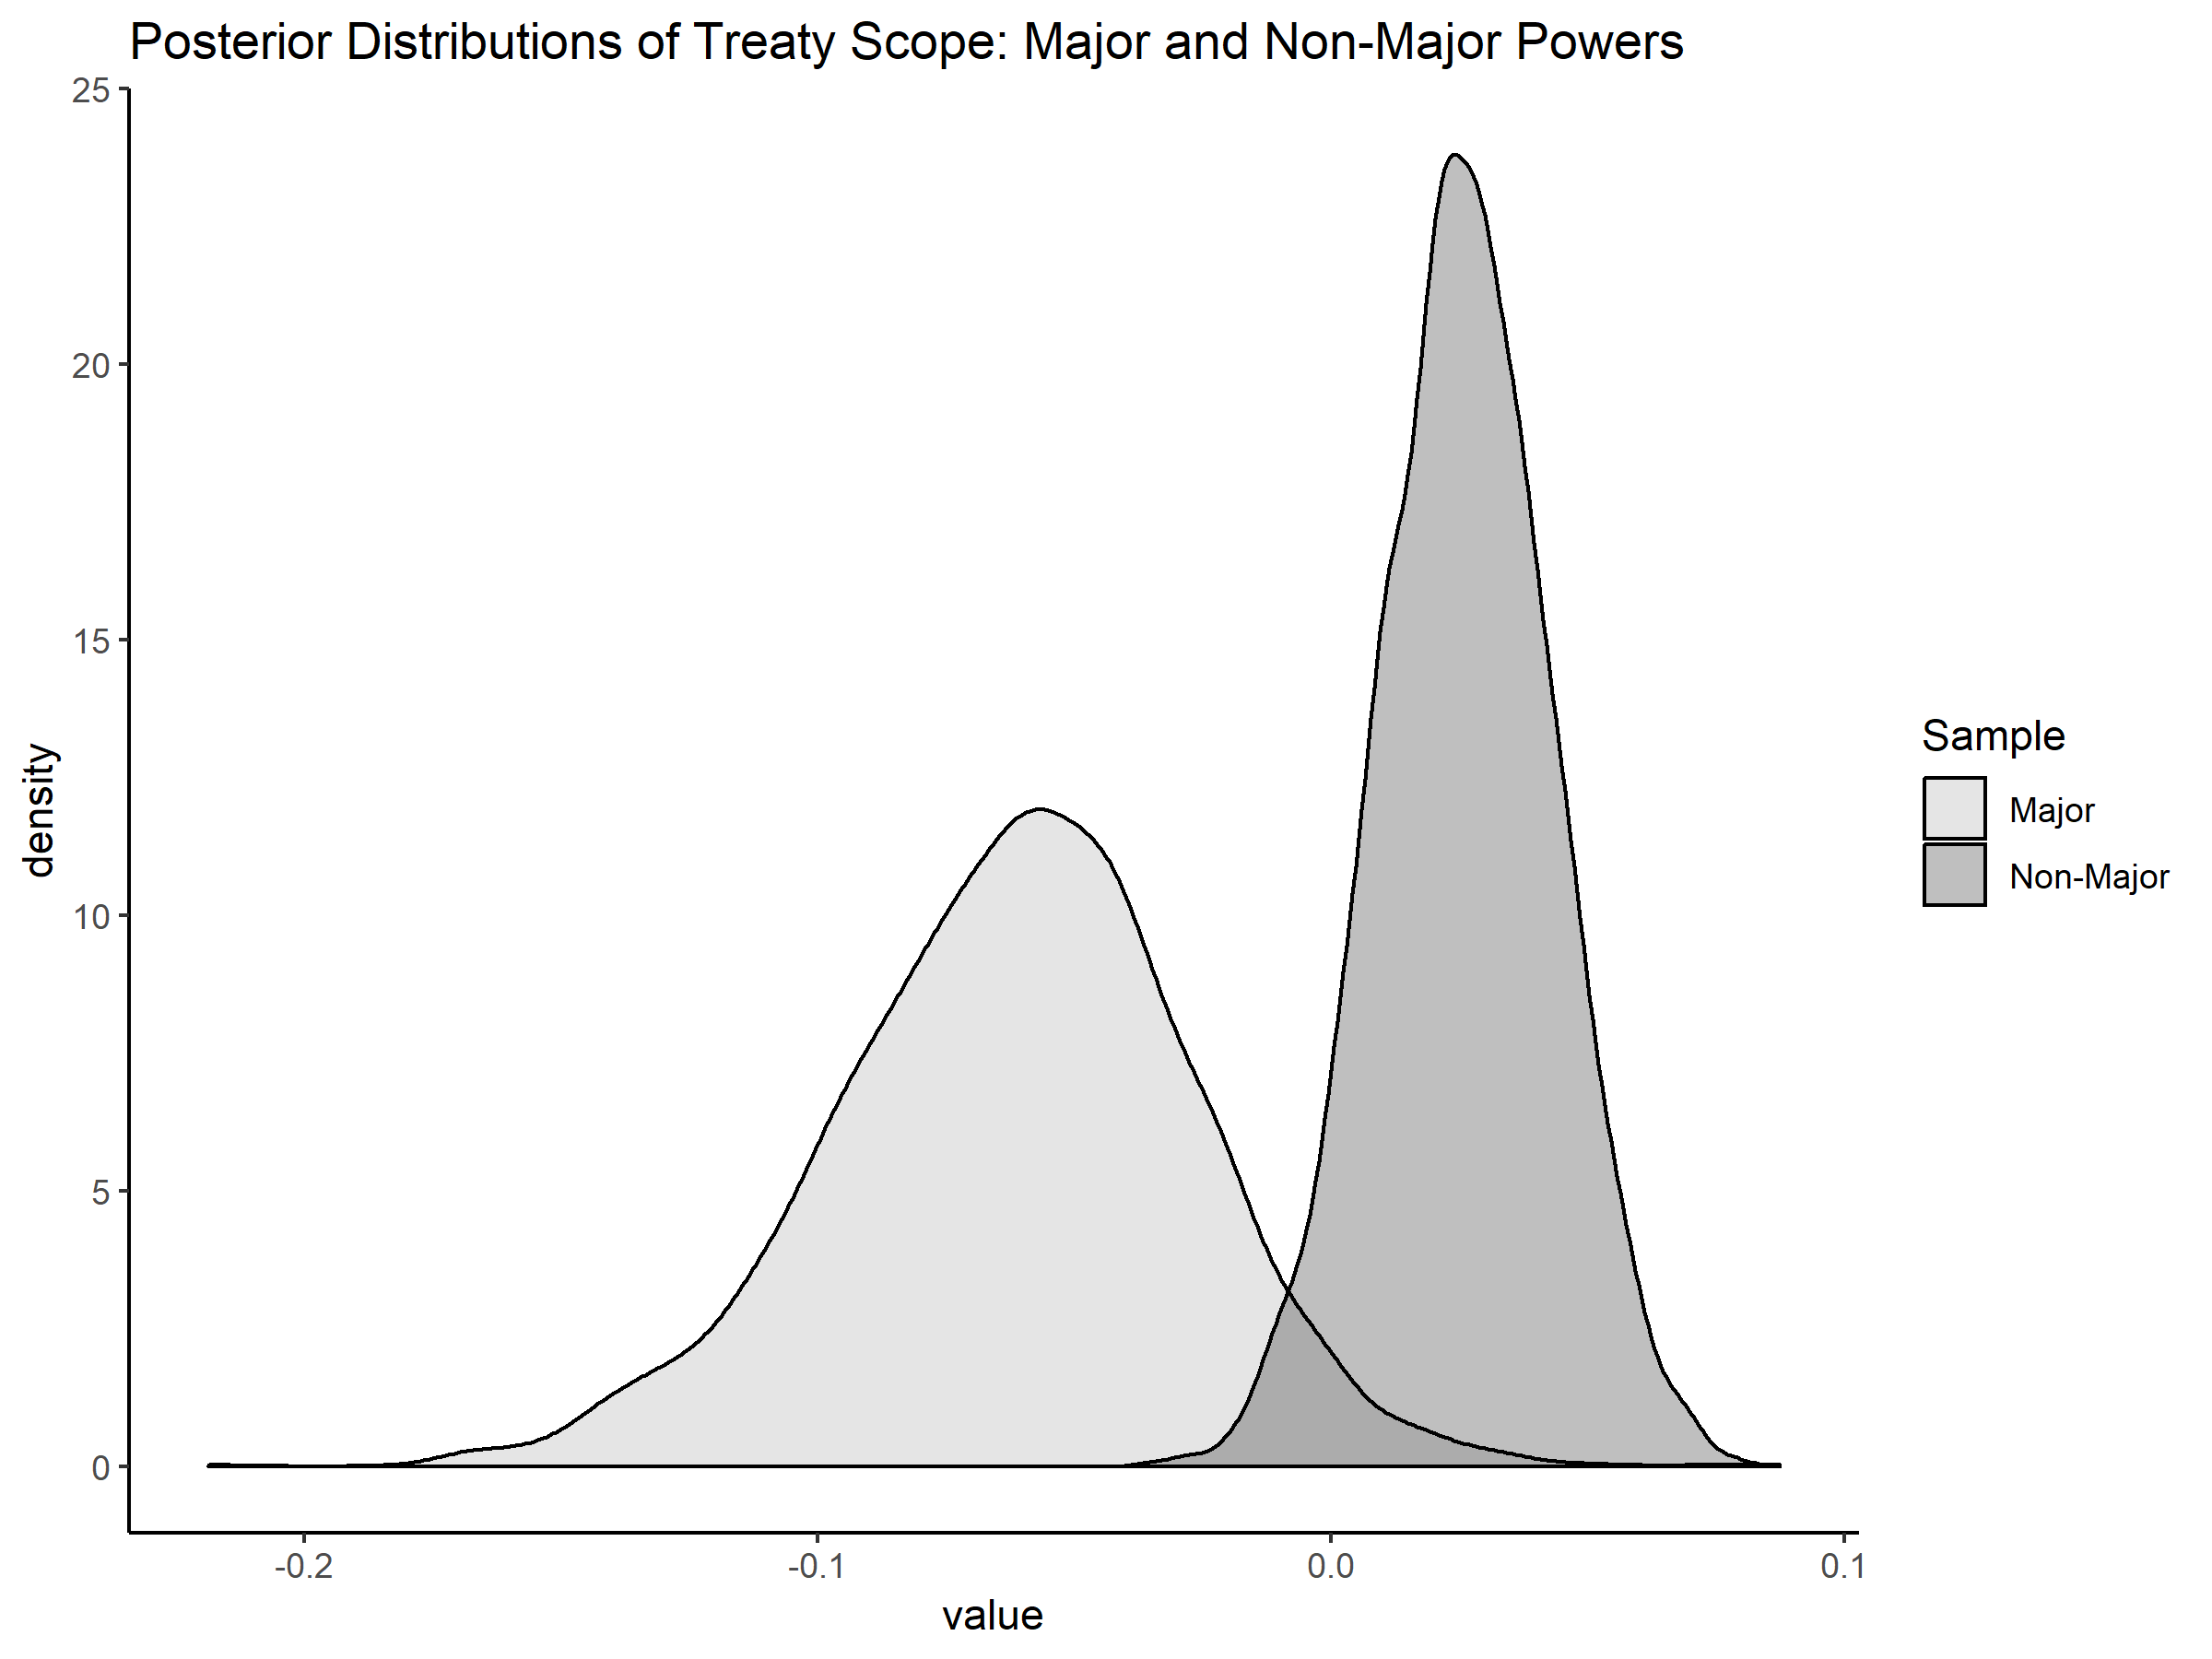
\includegraphics[width=0.95\textwidth]{../figures/scope-dens.png}
	\caption{Posterior density of treaty scope coefficient in major and non-major power samples, 1816 to 2007. 96\% of the major power posterior mass is negative. 94\% of the non-major power posterior mass is positive.}
	\label{fig:str-dens}
\end{figure}


\autoref{fig:str-dens} plots the full posterior density of the treaty scope coefficients in the major and minor power samples.\footnote{The smaller sample for major powers produces more variance in all the coefficient estimates.} 
96\% of the posterior mass for major powers is negative. 
94\% of the posterior mass for minor powers is positive. 


The preponderance of evidence matches the predictions of Hypotheses 1 and 2. 
For major powers, there is a 96\% chance increasing treaty scope is associated with lower growth in military spending. 
There is a 94\% chance greater treaty scope is associated with higher growth in military spending for non-major powers.


Of course seeing the expected sign on these two coefficients does not imply changing treaty scope is substantively important. 
To assess the substantive importance of a change in treaty scope, I compare the expected value of the coefficient to typical growth in military spending in each sample. 
Among major powers, the mean of the treaty scope coefficient is -0.05, and median growth in military expenditures is 0.04.\footnote{The median is a better summary of the dependent variable because large positive and negative outliers influence the mean.} 
So a one-unit increase in treaty scope more than offsets the typical annual growth in military spending. 
This change in spending is a plausible effect--- 5.1\% of the 2018 US defense budget was spent directly on NATO.\footnote{See this \href{https://www.iiss.org/blogs/military-balance/2018/07/us-and-nato-allies-costs-and-value}{blog post from the IISS}.} 


For non-major powers, the mean of the treaty scope coefficient is 0.03, and median growth in military expenditures is 0.06. 
Greater treaty scope increases growth in minor power military expenditures by about half of typical growth. 
In both the major and non-major power samples, the expected impact of higher treaty scope has a large substantive effect. \footnote{Of course, uncertainty in the posterior estimates includes larger and smaller effects.}


I also assess substantive importance by looking at patterns in the $\lambda$ parameters. 
Each $\lambda$ parameter measures the aggregate impact of treaty participation as function of treaty characteristics. 
If greater treaty scope has a large influence on alliances, there will be a clear trend in the mean of $\lambda$ across the range of alliance treaty scope.
We should observe a negative trend in the expected value of $\lambda$ as treaty scope increases in major power alliances. 
There will be a positive trend in $\lambda$ for non-major power alliances. 


\begin{figure}[htbp]
	\centering
		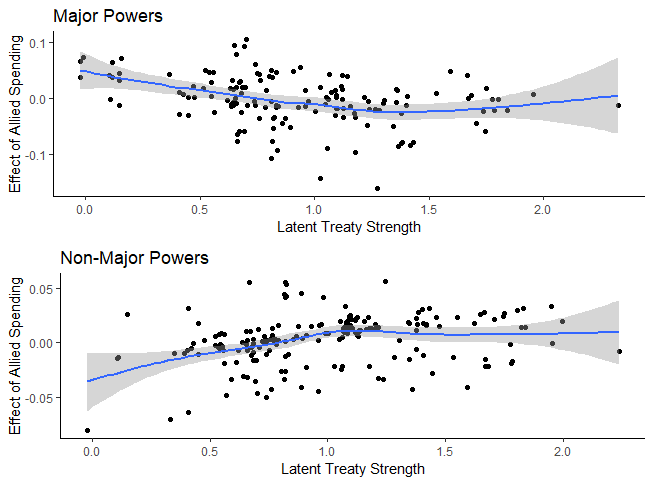
\includegraphics[width=0.95\textwidth]{../figures/lambda-ls-scatter.png}
	\caption{Scatter plots of trends in mean $\lambda$ parameters and treaty scope. $\lambda$ is the total impact of alliance participation on growth in military spending. The top panel is major powers, where this is a negative trend between $\lambda$ and treaty scope. In the bottom panel the same trend is positive for non-major powers. Trend lines estimated using linear regression.}
	\label{fig:lambda-ls-scatter}
\end{figure}


\autoref{fig:lambda-ls-scatter} plots the expected value of $\lambda$ against treaty scope in the two samples. 
In the major power sample, there is a negative trend in the scatter plot.
For non-major powers, the trend is positive.
The correlations between mean $\lambda$ and treaty scope are statistically significant in both samples. 


These trends match the underlying logic of Hypotheses 1 and 2. 
Limited treaties tend to increase growth in defense spending for major powers, but those associations fall as treaty scope increases. 
In non-major powers, shallow treaties tend to reduce growth in military spending, while deeper treaties usually have little impact or add to growth in military spending. 
Because other treaty characteristics and unmeasured factors also influence the $\lambda$ estimates, not all treaties conform to the expectations of decreasing or increasing growth in spending. 


Because $\lambda$ captures the total impact of an alliance, trends in these parameters across the range of treaty scope suggests that changing treaty scope has an important role. 
Even after accounting for other alliance characteristics, alliance strength drives the overall effect of allied spending down for major powers, and up for non-major powers. 
Alliance treaty scope is a key source of heterogeneity in how alliance participation impacts military spending. 
Making these comparisons underlines the benefits of the multilevel model estimates. 


While the statistical model estimates general associations, it does not show the underlying theoretical mechanisms. 
To illustrate the theoretical process, I offer evidence from US alliance politics in the next section.  
I focus on NATO--- the most important alliance in the international system. 


\section{NATO, treaty scope and Military Spending}


US foreign policy after World War II illustrates the tradeoff between entanglement and influence for major powers.
American choices in treaty design also had important consequences for junior partners. 
While forming alliances, the US balanced between fear of ``foreign entanglements'' and maintaining influence to check the USSR.
The Soviet threat allowed US policymakers to form a wide network of alliance treaties, but isolationists in the Senate weakened the formal promises in most treaties. 


% generally limited treaties 
Most US treaties contain few formal promises besides defense against aggression. 
These limited commitments led to additional defense outlays to support Washington's influence.  
NATO is an excellent example of these dynamics. 


% NATO 
After the end of World War II, the US sought a way to protect Europe from the USSR. 
Despite concern about Soviet intentions, isolationists in the US Senate feared an alliance would force America to intervene automatically if partners were attacked, bypassing the power of Congress to declare war \citep[pg. 280-1]{Acheson1969}.
Therefore Article V states that if one member is attacked the others ``will assist the Party or Parties so attacked by taking forthwith, individually and in concert with the other Parties, \emph{such action as it deems necessary} (emphasis mine).'' 
Military support was and is not guaranteed. 


The absence of automatic US involvement increased demand for reassurance by European allies. 
Europeans feared that if the Soviets invaded, the US would decide not to fight. 
Therefore, bilateral agreements on troop deployments provided reassurance and increased US influence. 


In 1950 West Germany formally requested clarification on whether an attack on US forces in Germany would be treated as an armed attack on the US- which the US said it would \citep[pg. 395]{Acheson1969}. 
A 1951 presentation by Dean Acheson to Dwight Eisenhower argued European allies ``fear the inconstancy of United States purpose in Europe. ... These European fears and apprehensions can only be overcome if we make the necessary full and active contribution in terms of both military forces and economic aid'' \citep[pg. 3]{Acheson1951}.  
But even after agreeing to deploy troops, US policymakers hoped Europeans would soon provide more for their own defense, while acknowledging the US ``should not dictate what they shall do'' \citep[pg. 2]{Johnson1950}. 


Isolationist fears of foreign entanglement also constrained formal scope in the NATO treaty. 
Many Senators also opposed military aid to Europe \citep[pg 285]{Acheson1969}, leading to more bilateral bargaining and aid through other channels. 
Due to the absence of formal sunk costs commitments in the NATO treaty, the US has limited leverage in NATO. 
NATO members have been free to reduce growth in defense spending with few consequences. 


In response, American policymakers from Eisenhower to Trump have attempted to browbeat NATO members into spending more. 
These shaming efforts have usually failed. 
Most European members of NATO have been unresponsive to changes in external threat and US defense spending \citep{PluemperNeumayer2015}. 


The US has threatened to leave NATO in response to this European ``free-riding,'' but those threats were not credible. 
During the Cold War, US interests in containing the USSR trumped irritation with allied free-riding.  
But without other costly treaty commitments to use as leverage, the US had few ways to check allied incentives to reduce growth in military spending. 


% add something on estimates from ML model
Estimates of the $\lambda$ parameter in the major and non-major power samples corroborate this reading of the NATO case. 
NATO is below the median in latent strength, so its formal promises are weaker than average among defense treaties. 
In the major power sample, NATO membership adds 0.04 to growth in military spending in expectation.
For non-major powers, NATO membership lowers growth in military expenditure by -0.006 in expectation.\footnote{
The UK and France are major powers from 1945 on, and Germany is coded as a major power by the Correlates of War after 1991. Therefore, these estimates may underestimate reduced growth in spending by NATO members, because all three of these states relied on US capability for protection. The positive growth in major power spending is driven by the US. In a future iteration of this paper, I will expand the classification of states to include superpowers.}


So the multilevel model estimates match prevalent narratives surrounding NATO.
US fear of entanglement led to a need for growth in military spending and limited bargaining leverage in alliance maintenance. 
European members still gained security, but retained the freedom of action to lower growth in defense spending.   
Evidence from NATO corroborates the expectations and process of my argument. 
These results have important implications for our understanding of alliance participation and military spending. 


\section{Discussion}


% Precise interpretation: compares alliances. Not treaty vs absence. 
My findings address the debate over whether alliance participation increases or decreases military spending. 
Dissension between the force multiplier and foreign entanglement views of alliances is based on competing claims about the purposes of alliances. 
This dispute omits crucial differences between states and alliances. 


My findings and argument suggest claims alliance participation only increases or decreases military spending are inappropriate. 
Major and non-major powers respond differently to alliance participation, because they use treaties for different purposes. 
Alliance treaty design also has different ramifications for more or less capable states. 


While alliance participation tends to increase major power military spending, greater treaty scope reduces that growth in spending. 
Conversely, the tendency of non-major powers to lower growth in military spending due to alliance participation is attenuated by increasing treaty scope. 
Therefore, my argument and evidence expose the limits of the conventional wisdom on this question, and clarifies where each perspective can be applied. 


% Link for force multiplier and foreign entanglement
The force multiplier perspective applies best to non-major powers. 
But these states cannot reduce growth in military spending in all alliances, because deep treaties constrain their freedom of action.
The foreign entanglement prediction holds for major powers. 
But additional entanglement in a deep treaty provides more influence, which attenuates the positive correlation between alliance participation and growth in military spending. 


My findings and argument connect previously separate components of the political economy of alliances. 
The first component is work on issue linkage politics in alliances \citep{Poast2012, Poast2013, Johnson2015}.
The second is the arms-alliances tradeoff, or the link between alliance participation and military spending \citep{Morrow1993}. 
By using issue linkages and treaty scope to explain when alliance participation increases or decreases military spending, my work provides a more unified perspective on the political economy of alliances.  


How do these findings compare to prior evidence on alliance participation and military spending? 
Connecting my findings with earlier evidence requires renewed attention to specific and general research designs. 
General studies compare states in a particular kind of alliances to those without such an alliance. 
Specific studies estimate responsiveness to allied military spending in a few treaties. 


My research design emulates specific studies by estimating the unique impact of participation in individual treaties. 
I then use alliance treaty design to explain variation in how treaty participation impacts growth in military spending.
Differences in alliances give general estimates that are not tied to individual treaties.  


The key coefficient estimates compare deep and shallow treaties. 
The alliance-level coefficient estimates are like marginal effects- increasing treaty scope alters the effect of alliance participation.
This captures the general consequences of participating in a particular treaty. 
Therefore, my results encompass specific and general studies in a unified framework. 
I provide estimates to infer and compare the impact of individual treaties and general differences between treaties. 


% limitations of RD
This paper has several limitations.
The argument does not address the domestic political economy of military spending. 
My argument reduces domestic politics to an assumption that military spending has opportunity costs, which are decreasing in state size. 
Domestic politics shapes how states define their foreign policy interests and the tools they use to pursue those interests \citep{Fordham1998, Fordham2011, Narizny2007}.
At the moment, my argument treats foreign policy interests as given.  


In the research design, the COW measures of military spending contain substantial measurement error. 
There is also a great deal of missing data in the 1816--2007 time frame of this study. 
I plan to check the robustness of my results to these issues by adding measurement error to the outcome and imputing missing data.


The multilevel model only incorporates time-invariant alliance characteristics, save for changing capabilities in the membership matrix. 
So I measure share of democratic members and the number of members at time of formation. 
Allowing time-varying alliance characteristics might improve the statistical model, but would require altering the model structure. 


My findings also only address formal issue linkages. 
The measure of treaty strength only includes formal promises, in part because informal issue linkages around military spending are hard to observe. 
As a result, my test of treaty scope and the associated issue linkages is probably conservative--- it does not capture phenomena my argument expects should have a similar effect. 


% Strategic treaty design
Strategic alliance design is the last major weakness of the research design. 
Non-random selection into different kinds of alliances might produce systematic differences between members that are no adjusted for in my statistical model. 
I attempted to control for correlates of alliance treaty scope, especially democracy, but oversights are possible. 


Despite these limitations, I believe the argument and results provide valuable insights about alliance participation and military spending. 
I explain when alliance participation is associated with more or less growth in military spending, addressing a debate between the force multiplier and foreign entanglement views of alliances. 
Whether alliance participation increases or decreases military spending depends on state capability and alliance treaty scope. 
For major powers, greater treaty scope leads to lower growth in spending. 
Non-major power growth in spending is positively correlated with alliance treaty scope. 
I provide evidence for these predictions using a new measure of alliance treaty scope and a multilevel model. 
The argument and findings have implications for scholars and policymakers. 



\section{Conclusion}


% Start conclusion
There are several ways scholars can build on these results. 
First, my findings reinforce calls to pay attention to heterogeneity among alliances \citep{Leeds2003, DigiuseppePoast2016}.
Scholars should also consider the distributional consequences of changes in military spending and assess a wider range of empirical evidence. 


% Add paragraph on distributional consequences.
Changes in military spending from alliance participation have important distributional consequences. 
By altering growth in military spending, the design of international alliances alters the domestic political economy of member states. 
But the domestic economic consequences of alliance politics are not well understood. 


% Next steps: extend argument to other treaty characteristics
Besides exploring the domestic political economy of alliance participation, future work should extend my argument to other alliance characteristics. 
If major and non-major powers employ alliances for different ends, then other alliance characteristics may have different impacts on military spending. 
Other treaty design considerations, such as asymmetric obligations, should have different effects for major and non-major powers. 


% Next steps: More interp of lambdas
Another task for future research is making more detailed comparisons of the $\lambda$ parameters. 
Each $\lambda$ captures the aggregate impact of alliance participation for individual treaties.
Due to space limitations, this paper offers a cursory treatment of these estimates. 
As such, these parameters are a novel measurement, and additional evidence of when alliance participation increases or decreases military spending. 


% Case studies
The multilevel model estimates alone cannot establish causality \citep{Seawright2016}. 
I provided a brief illustration using NATO, but selected that case for its illustrative value and policy importance, not for inference. 
This leaves room for more precise selection of cases to corroborate the regression results. 
One possible design is using the five largest and smallest $\lambda$ values for major and minor powers to select cases. 
Process tracing in these cases could then examine theoretical mechanisms and validate measurement \citep{Seawright2016}. 


% ML model and other cases of multiple membership 
Beyond the immediate issue of alliance participation and military spending, the research design in this paper could apply to other international relations questions.
If scholars are interested in a class of international organizations where membership in multiple organizations is not nested and institutional characteristics generate heterogeneous effects, the multilevel model addresses all of these concerns.
For example, international political economy scholars could apply this model to trade agreements. 
Studies of international law could examine the impact of membership in different conventions and international organizations on human rights. 


% The argument indicates tradeoff
Besides their scholarly value, the argument and evidence have important consequences for policy debates. 
The tradeoffs major and non-major powers face in alliance treaty design can guide our understanding of why some treaties lead to ``free-riding'' and potential responses. 
US policymakers must consider the major power tradeoff between foreign entanglement and influence in deep treaties. 
Greater influence can limit allied free-riding, but it requires deeper engagement abroad. 


% Implications for policy. 
The United States is currently wrestling with the implications of differences in treaty scope. 
Washington has often decried ``free-riding'' by allies who provide too little for their own defense \citep{Lanoszka2015}. 
But allies are able to free-ride because the US makes relatively limited formal alliance commitments. 
``Entangling alliances'' may provide more influence to curb falling allied defense spending. 

 
Therefore, growing institutionalization of NATO, including the agreement for all allies to spend at least 2\% of GDP on defense, may be effective.
A deeper formal structure will tie the US more closely to Europe, but it is probably a better check on allied free-riding than the usual verbal exhortations. 
Threatening to leave the alliance is not credible and risks undermining US gains from alliances. 
So long as formal ties are relatively limited, US leaders will lack leverage in intra-alliance bargaining. 


The US could use deeper formal commitments as a substitute for greater defense effort in reassuring allies.
The danger is that increasing treaty scope could create a situation where obligations exceed capabilities \citep{Kennedy1987}. 
Emboldening junior partners with a deep treaty might have deterrent value \citep{Bensonetal2014}, or increase the risk of conflict \citep{Benson2012}.
Every change in alliance treaty scope generates different risks and tradeoffs--- policymakers must strike an appropriate balance. 
 

% tie it all together
Alliance participation will not uniformly increase or decrease military spending. 
Rather, the connection between alliance participation and military expenditures depends on treaty scope and state capability.  
Both the force multiplier and foreign entanglement views of alliance participation are correct, each in different circumstances. 




\singlespace
 
\bibliography{../../MasterBibliography} 





\end{document}
